

%%%%%%%%%%%%%%%%%%%%%%%% ADD CONTENT %%%%%%%%%%%%%%%%%%%%%%
\section{Introduction to programming}
\begin{frame}{\insertsectionnumber{ |} Command-line basics (*nix)}

\hspace*{-0.5cm}\textbf{Basic commands} \\
\vspace*{0.15cm}\begin{tabular}{p{0.75cm} p{6cm} p{3.5cm}}
\textbf{command} & \textbf{~~example} & \textbf{description} \\
ls & \Verb+ ls -ltrh + & \ul{l}i\ul{s}t directory contents (in long format, newest last) \\
cd & \Verb+ cd ../mydir/mysubdir + & \ul{c}hange \ul{d}irectory (up one level, down two) \\
rm & \Verb+ rm delete-this.txt and-all-these.* + & \ul{r}e\ul{m}ove file(s) \\
mv & \Verb+ mv rename-this.txt to-this.txt + & \ul{m}o\ul{v}e (rename) file(s) \\
mkdir & \Verb+ mkdir ./new-directory + & \ul{m}a\ul{k}e a new (empty) \ul{dir}ectory  \\
cp & \Verb+ cp this.txt ./new-dir/to-this.txt + & \ul{c}o\ul{p}y file (possibly to new location) \\
\end{tabular}


\vspace*{0.35cm}\hspace*{-0.5cm}\textbf{Linux c-line tools} \\
\vspace*{0.15cm}\begin{tabular}{p{0.75cm} p{6cm} p{3.5cm}}
\textbf{tool} & \textbf{~~example} & \textbf{description} \\
pwd & \Verb+ pwd + & Find out what your current \ul{p}ersonal \ul{w}orking \ul{d}irectory is \\
sed & \Verb+ sed -e `s/a/b/g'+ & \ul{s}tream \ul{ed}itor, swap `a' for `b' \\
awk & \Verb+ awk `\{print \$2, \$3\}'+ & print fields 2 \& 3 from file/stream \\
\end{tabular}

\vspace*{0.35cm}\hspace*{-0.5cm}\textbf{Other packages \& utilities} \\
\vspace*{0.15cm}\begin{tabular}{p{0.75cm} p{6cm} p{3.5cm}}
\textbf{package} & \textbf{~~example} & \textbf{description} \\
pdflatex & \Verb+ pdflatex myfile.tex + & compile \LaTeX ~document \\
git & \Verb+ git clone golledni/WinterSchool + & Make a local copy of a github repository \\
\end{tabular}


\end{frame}

%%%%%%%%%%%%%%%%%%%%%%%%

\begin{frame}[fragile]{\insertsectionnumber{ |} Simple (bash) shell scripting}



\begin{columns}
\column[c]{7.5cm}
\begin{itemize}

\begin{beamerboxesrounded}[lower=gray,shadow=true]{
\item We can combine many simple commands, tools, and utilities to achieve more complex tasks
}
\end{beamerboxesrounded}
\end{itemize}
\end{columns}

\vspace*{1cm}\begin{lstlisting}
pwd
/home/golledni/MEGA/Work/AntSciPlat/WinterSchool

pwd | sed -e `s/\// /g' | awk `{print "Today my",$1,"is the",$NF}'
Today my home is the WinterSchool
\end{lstlisting}


\begin{beamerboxesrounded}[lower=gray,shadow=true]{
\vspace*{0.5cm}
}
\end{beamerboxesrounded}

\end{frame}


%%%%%%%%%%%%%%%%%%%%%%%%

\begin{frame}{\insertsectionnumber{ |} Simple (bash) shell scripting}

\begin{columns}
\column[c]{7.5cm}
\begin{itemize}

\begin{beamerboxesrounded}[lower=gray,shadow=true]{
\item But to do anything more complex than simple pipes we probably want to write a script file to contain our sequence of commands:
}
\end{beamerboxesrounded}

\end{itemize}
\end{columns}

\vspace*{0.5cm}\centering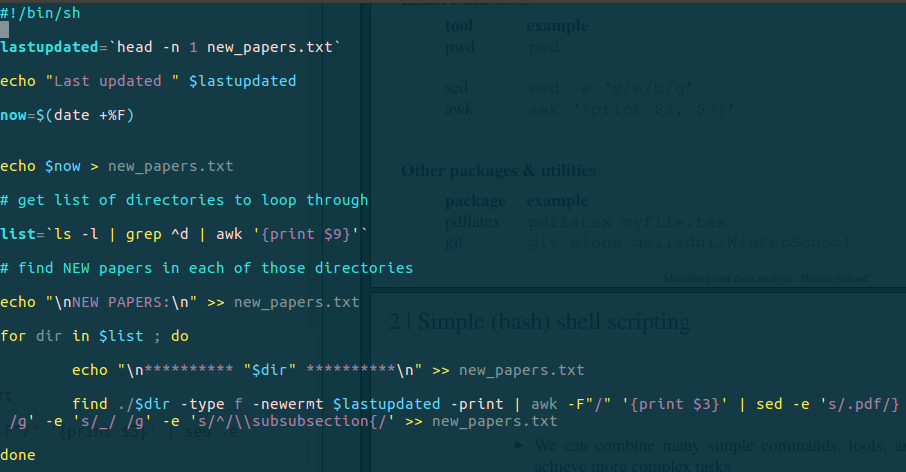
\includegraphics[width=10cm]{./images/sh-script.png}\\

%\begin{beamerboxesrounded}[lower=gray,shadow=true]{
%\vspace*{0.5cm}
%\item 
%}
%\end{beamerboxesrounded}
%
%\begin{beamerboxesrounded}[lower=gray,shadow=true]{
%\vspace*{0.5cm}
%\item 
%}
%\end{beamerboxesrounded}




\end{frame}



%%%%%%%%%%%%%%%%%%%%%%%% END CONTENT %%%%%%%%%%%%%%%%%%%%%%
